\section{Geo-zones}
Geo-zone visual representation can be used as the first example of GIS web component possibilities. Geo-zones represent simple geographical polygons that can ``guard'' machine movements and help to store intersection events. They can be used to determine whether machine is in the right place in particular time or whether the route is performing well.

In Transmirror project Geo-zones have been used to determine the count of performed route circles on a daily basis for route vehicles. It helps the manager to control the amount of vehicle fuel usage. It also give an ability to quickly analyse whether the driver is on time on route stoppages and whether the important stoppages were not bypassed.

Geo-zones web UI has been incorporated to the Transmirror tree menu as ``Гео-зони (web)'' item under ``Довідники'' umbrella. Menu item double-clicking invokes the entity-centre with GIS web view. After running the query for the first time by clicking on the Run button all existing Geo-zones are shown as small purple graphic primitives. After Run action has performed all primitives are also fitted to the bounds of visible map view automatically. In case when not all Geo-zones are visible (due to zooming / panning activities) the user can do manual ``Fit To Bounds'' action by clicking appropriate button (figure~\ref{fig:01}).

\begin{figure}[H]
\centering
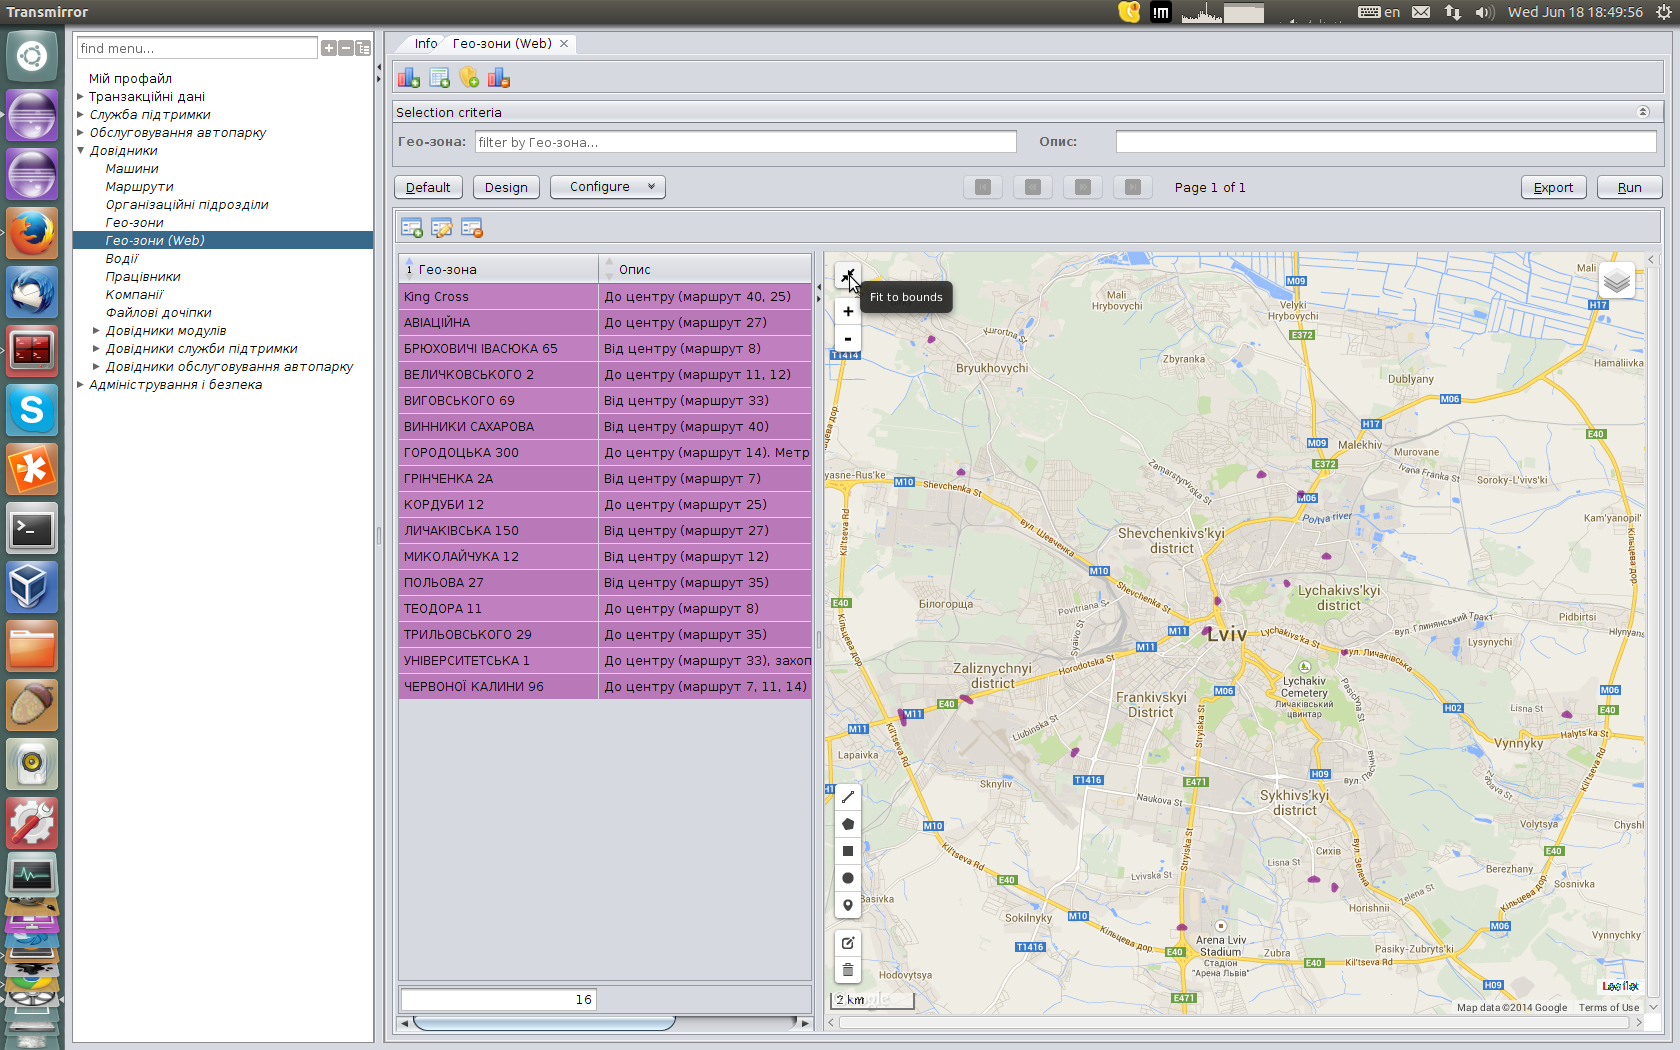
\includegraphics[width=\linewidth]{chapters/01-geozones/images/01-all-geo-zones-using-fit-to-bounds-button.png}
\caption{Positioning of all Geo-zones using ``Fit To Bounds'' button}\label{fig:01}
\end{figure}

\newpage
The necessary details can be viewed using zooming feature. Zooming can be done traditionally with mouse wheel button and a pair of zooming buttons ``+'' and ``-''. Also the user can press SHIFT button in conjuction with mouse selection and it works as a convenient zooming method (figure~\ref{fig:02}). It is very useful when some specific rectagular geo-area is interested in. 

\begin{figure}[H]
\centering
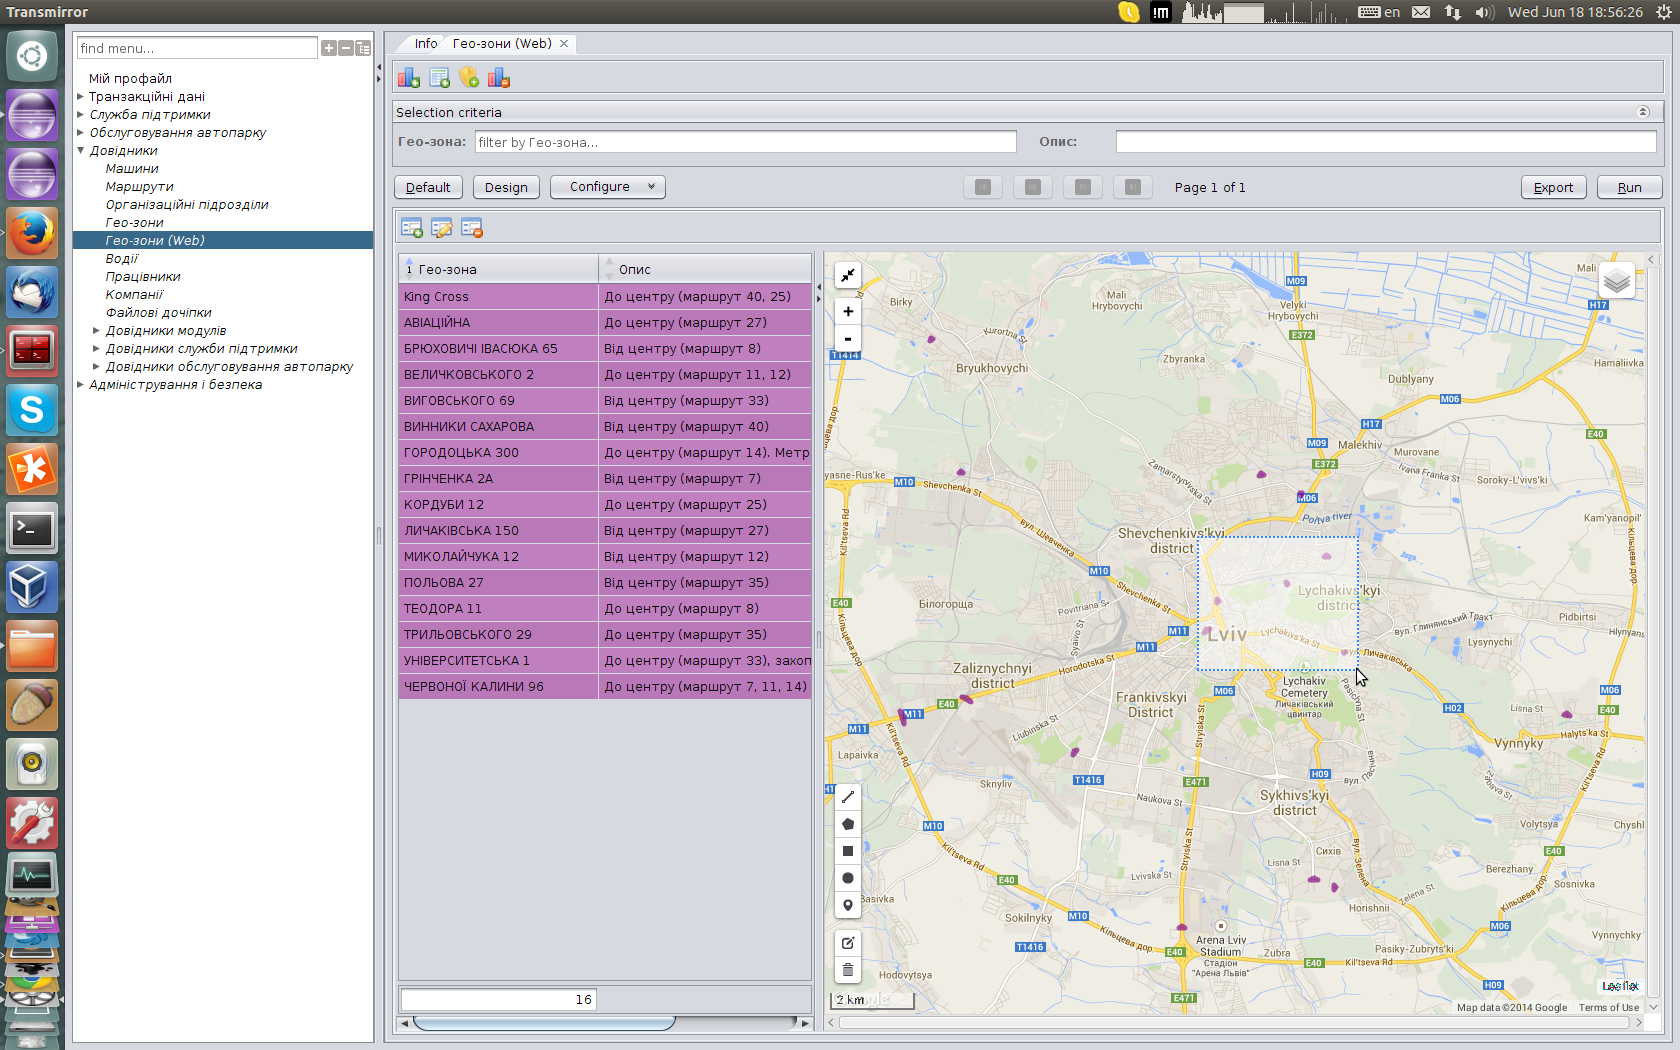
\includegraphics[width=\linewidth]{chapters/01-geozones/images/02-part-of-geo-zones-using-shift+selection-zoom.png}
\caption{Zooming with SHIFT-selection: showing a part of Geo-zones}\label{fig:02}
\end{figure}

\newpage
The result of zooming shows that example Geo-zones has been represented as triangles (figure~\ref{fig:03}). But actually, directed vector-like Geo-zones have been used for Transmirror project. The triangular shape has been only chosen to express the direction in which the vehicle should move through the Geo-zone to make an intersection. It resolves a common problem with GIS software -- intersection of Geo-zones by moving in opposite ways on the same road section. No distiction can be provided if Geo-zone has no ``direction'' concept assigned.

The shapes are not limited only by triangles -- complex polygons or circles can be used as well (see later figure~\ref{fig:07}). This is handy when a precise geozone shape of some specific nature is needed (for e.g. parking area or field).

The another convenient way to zoom to some concrete node is to just click on it (figure~\ref{fig:03}).

\begin{figure}[H]
\centering
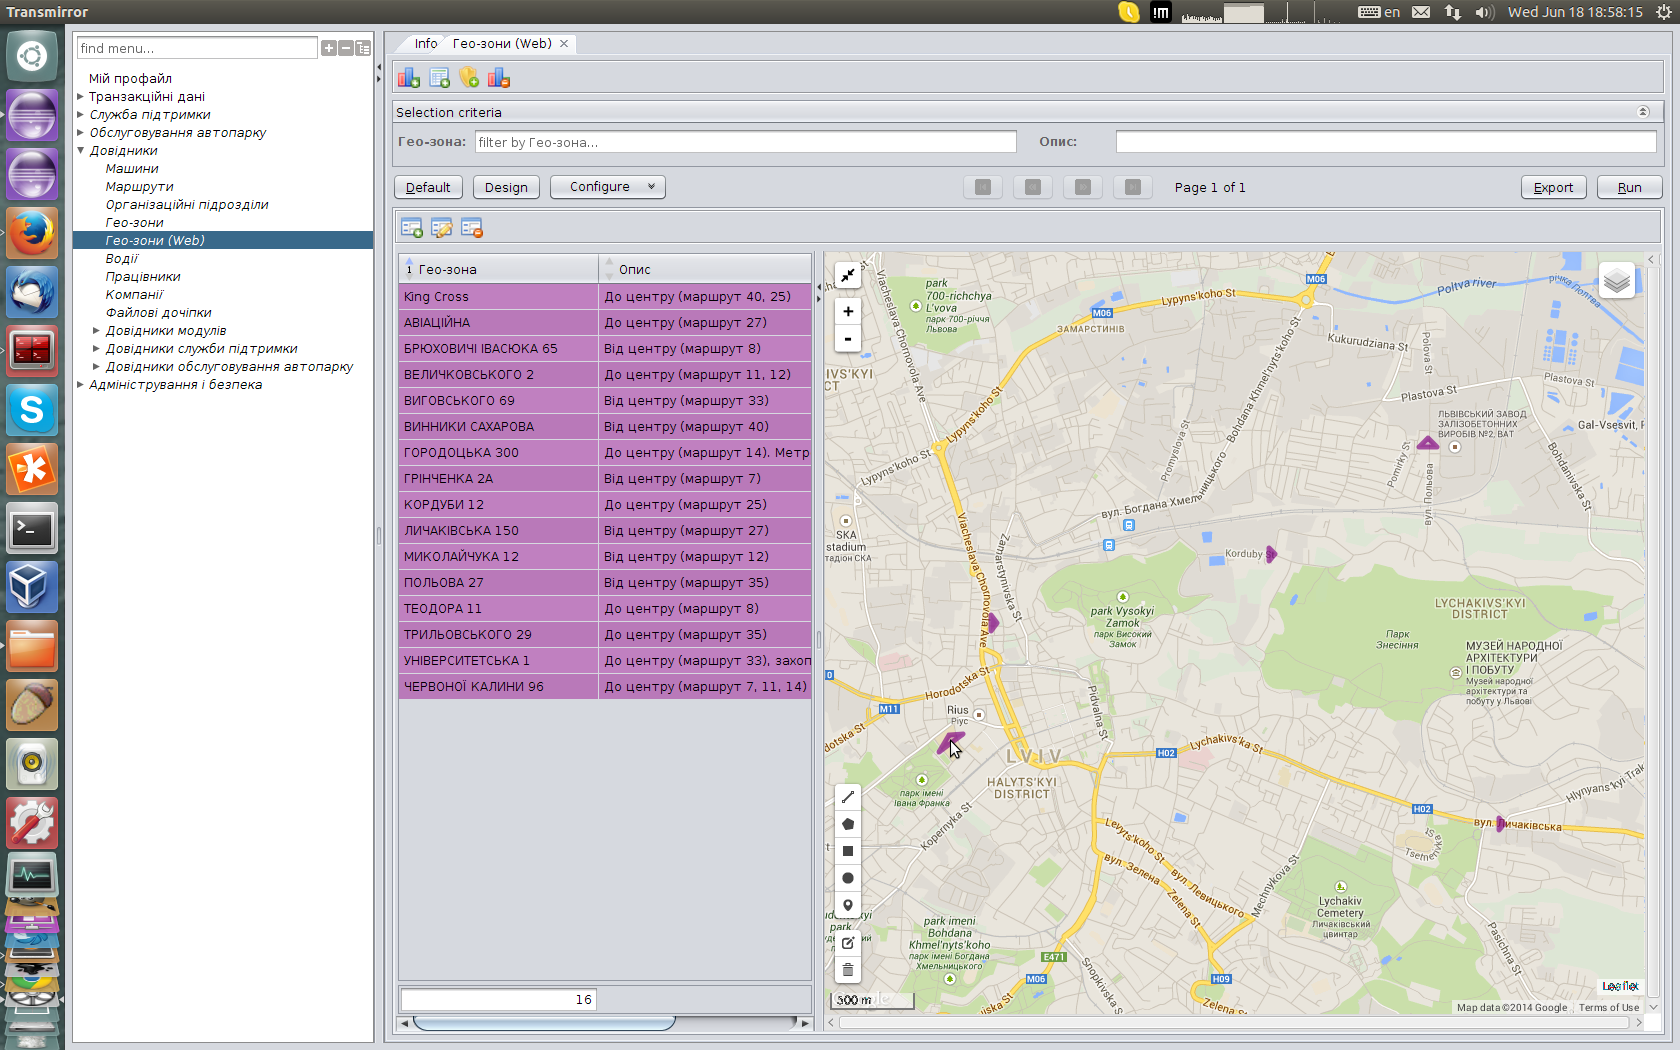
\includegraphics[width=\linewidth]{chapters/01-geozones/images/03-part-of-geo-zones-with-particular-item-selection-by-clicking.png}
\caption{Part of Geo-zones with particular item selection by clicking}\label{fig:03}
\end{figure}

\newpage
Clicking on triangle will fit it to the bounds of the map and will show the detailed popup information (figure~\ref{fig:04}). The table also will synchronise with the selected item (appropriate table row will also be selected). At this stage the table component is the regular Entity Grid Inspector that is used in all TG client applications. The development of Web-enabled EGI is on upcoming schedule.

\begin{figure}[H]
\centering
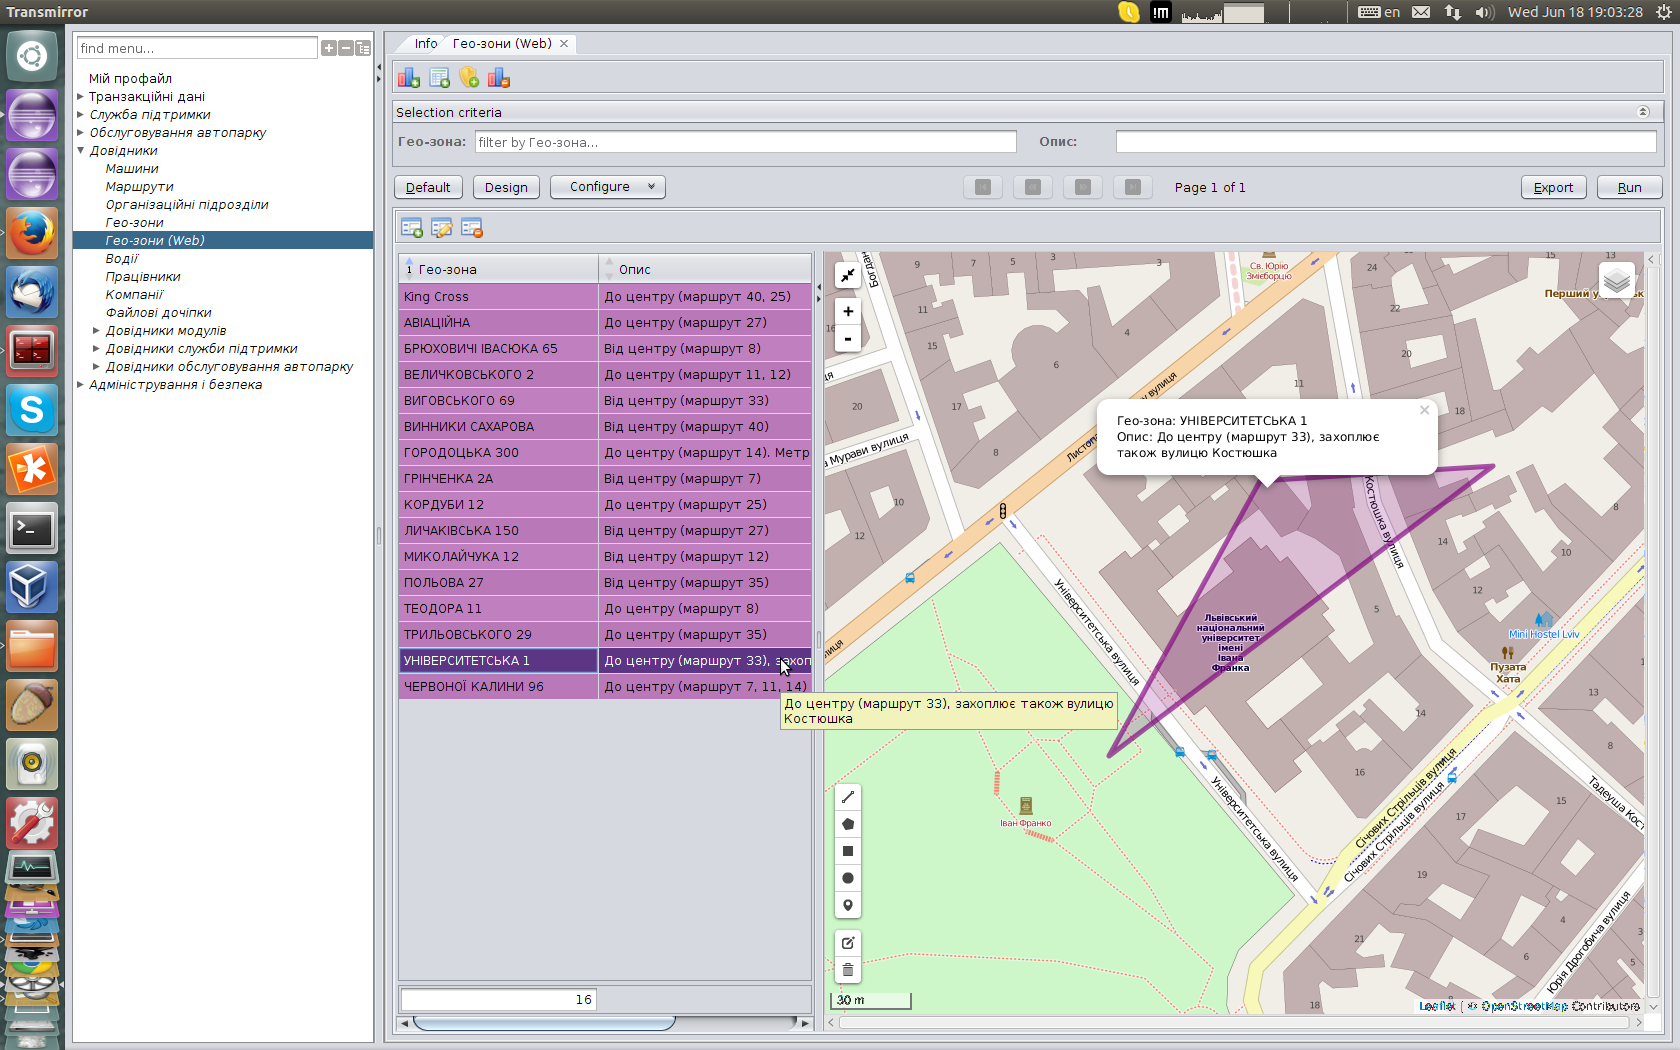
\includegraphics[width=\linewidth]{chapters/01-geozones/images/04-selected-geo-zone-and-synchronised-with-grid.png}
\caption{The Geo-zone has been selected and synchronised with Entity Grid Inspector}\label{fig:04}
\end{figure}

\newpage
Editing of Geo-zones is also supported by dragging polygon corners (figure~\ref{fig:05}). Appropriate shape can be formed with arbitrary number of corners -- the ``greyed-out'' corners (in the middle of the line segments) should be used to extend number of corners. The changes can be simply discarded if needed using ``Cancel" button or saved with ''Save" button.

\begin{figure}[H]
\centering
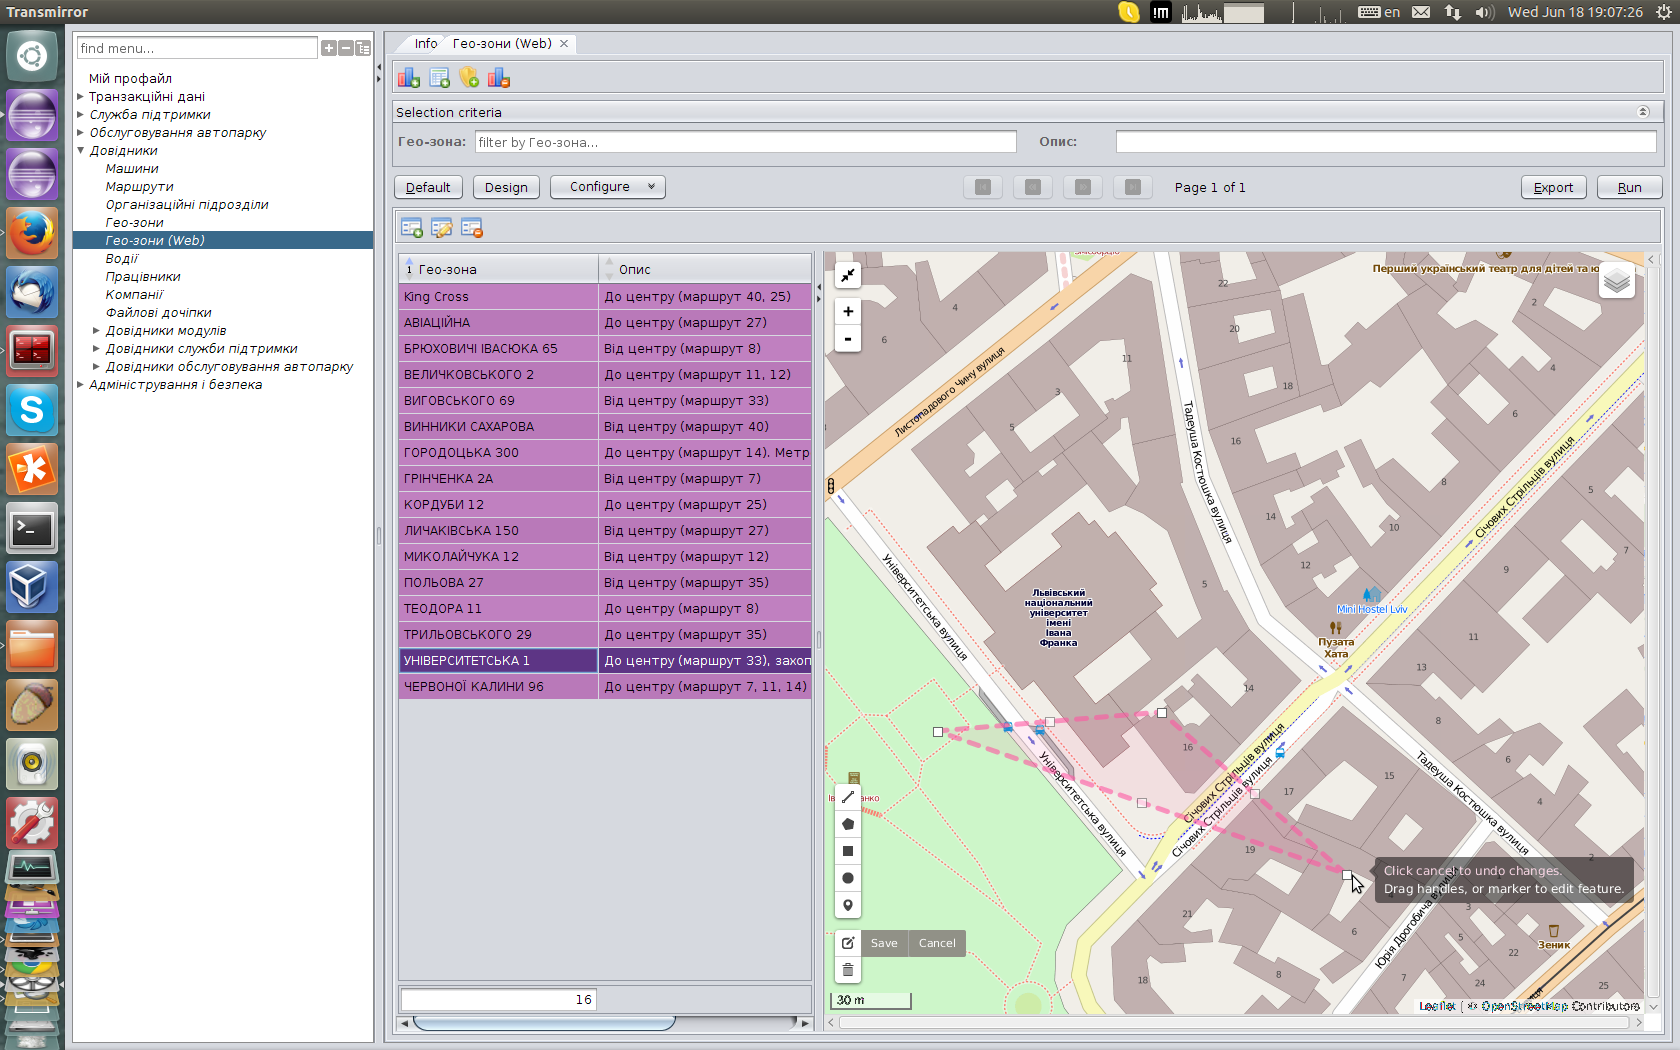
\includegraphics[width=\linewidth]{chapters/01-geozones/images/05-editing-geo-zone-using-graphical-interface.png}
\caption{Geo-zone editing using graphical interface}\label{fig:05}
\end{figure}

\newpage
The result of editing is a regular shape (figure~\ref{fig:06}) that can be used exactly the same as the previous version.

\begin{figure}[H]
\centering
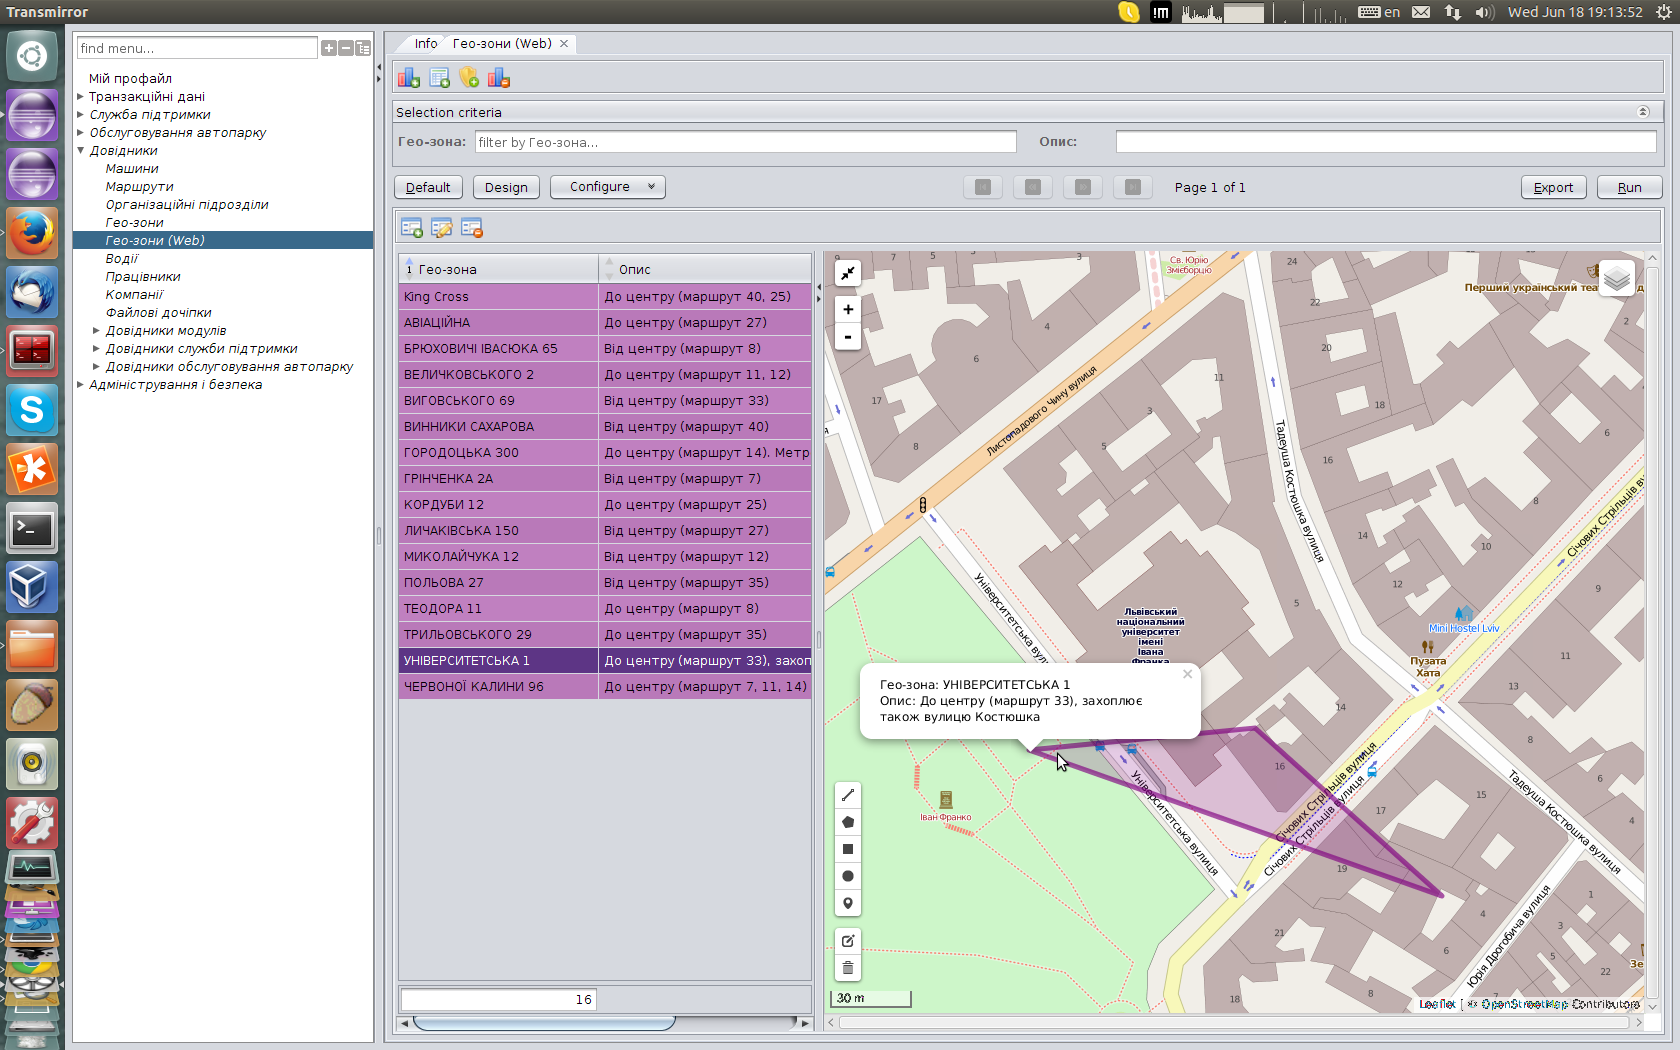
\includegraphics[width=\linewidth]{chapters/01-geozones/images/06-edited-geo-zone.png}
\caption{Edited Geo-zone}\label{fig:06}
\end{figure}

\newpage
As has been mentioned before, complex shapes can be used (figure~\ref{fig:07}). These include circles, rectangles or polygons. The area amount is also calculated during polygon editing.

\begin{figure}[H]
\centering
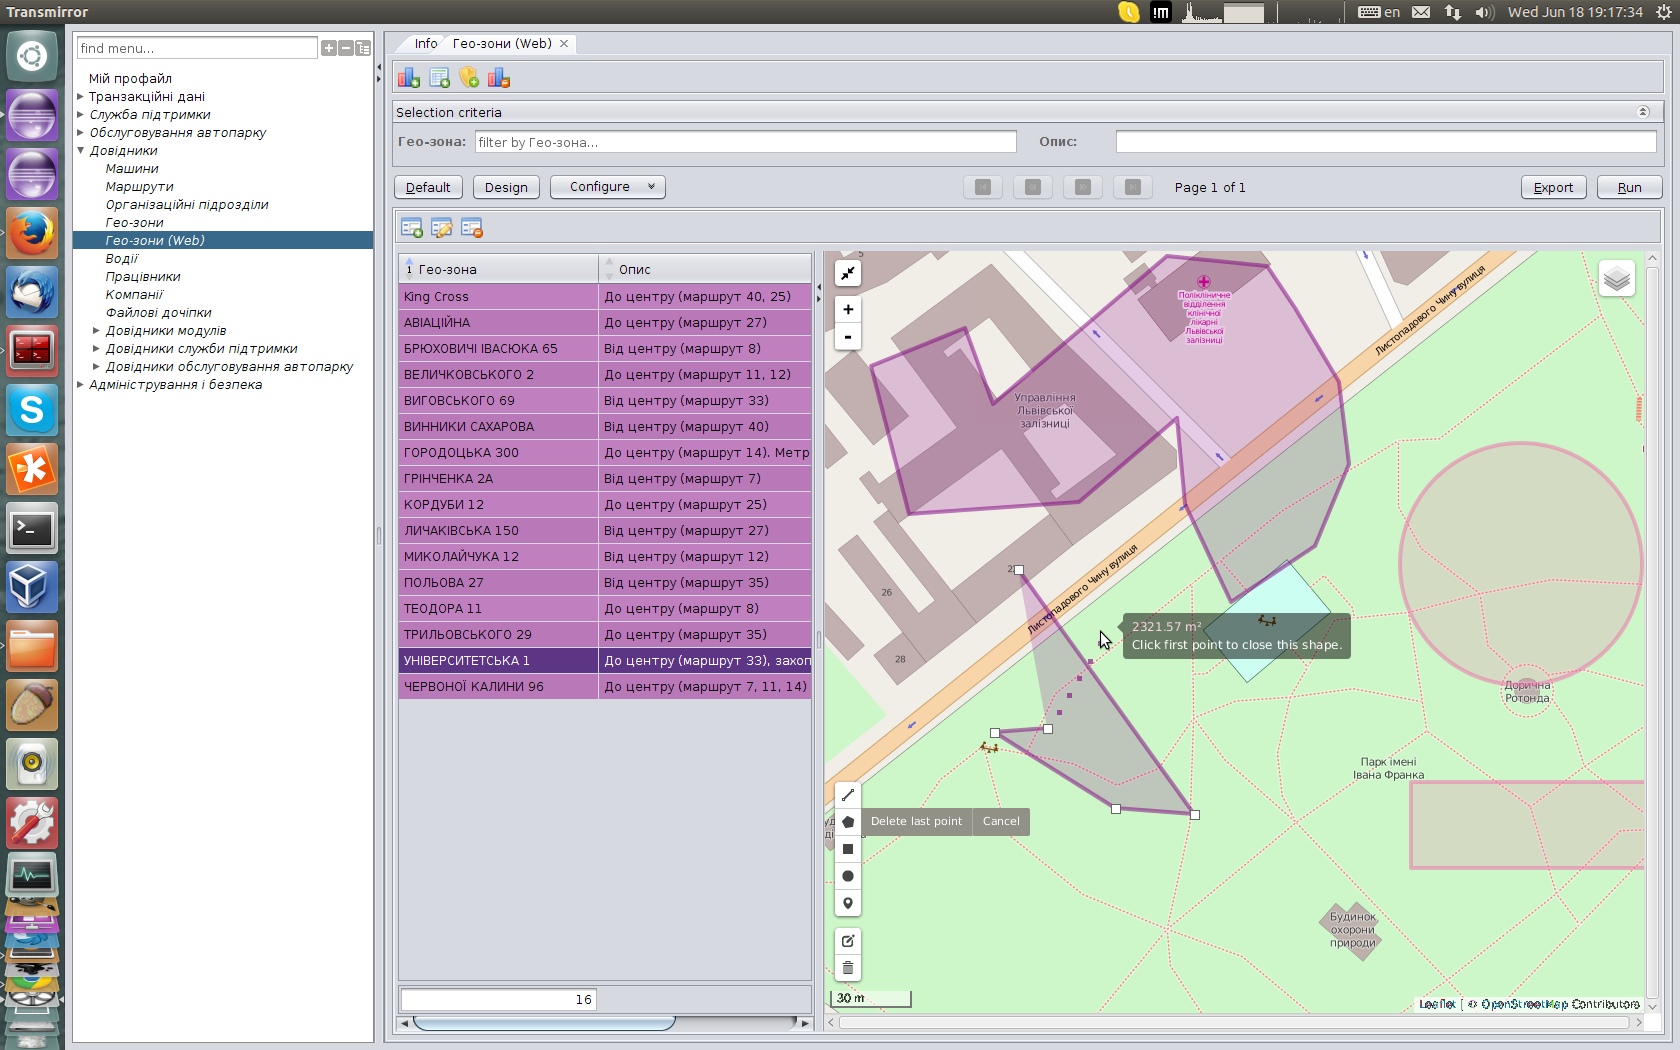
\includegraphics[width=\linewidth]{chapters/01-geozones/images/07-creating-new-complex-geo-zones.png}
\caption{Creating new complex Geo-zones}\label{fig:07}
\end{figure}

\newpage
Validation for the shape is necessary to make possible only meaninful Geo-zones (the edges should not cross). This is also done during editing as the area amount calculation (figure~\ref{fig:08}).

\begin{figure}[H]
\centering
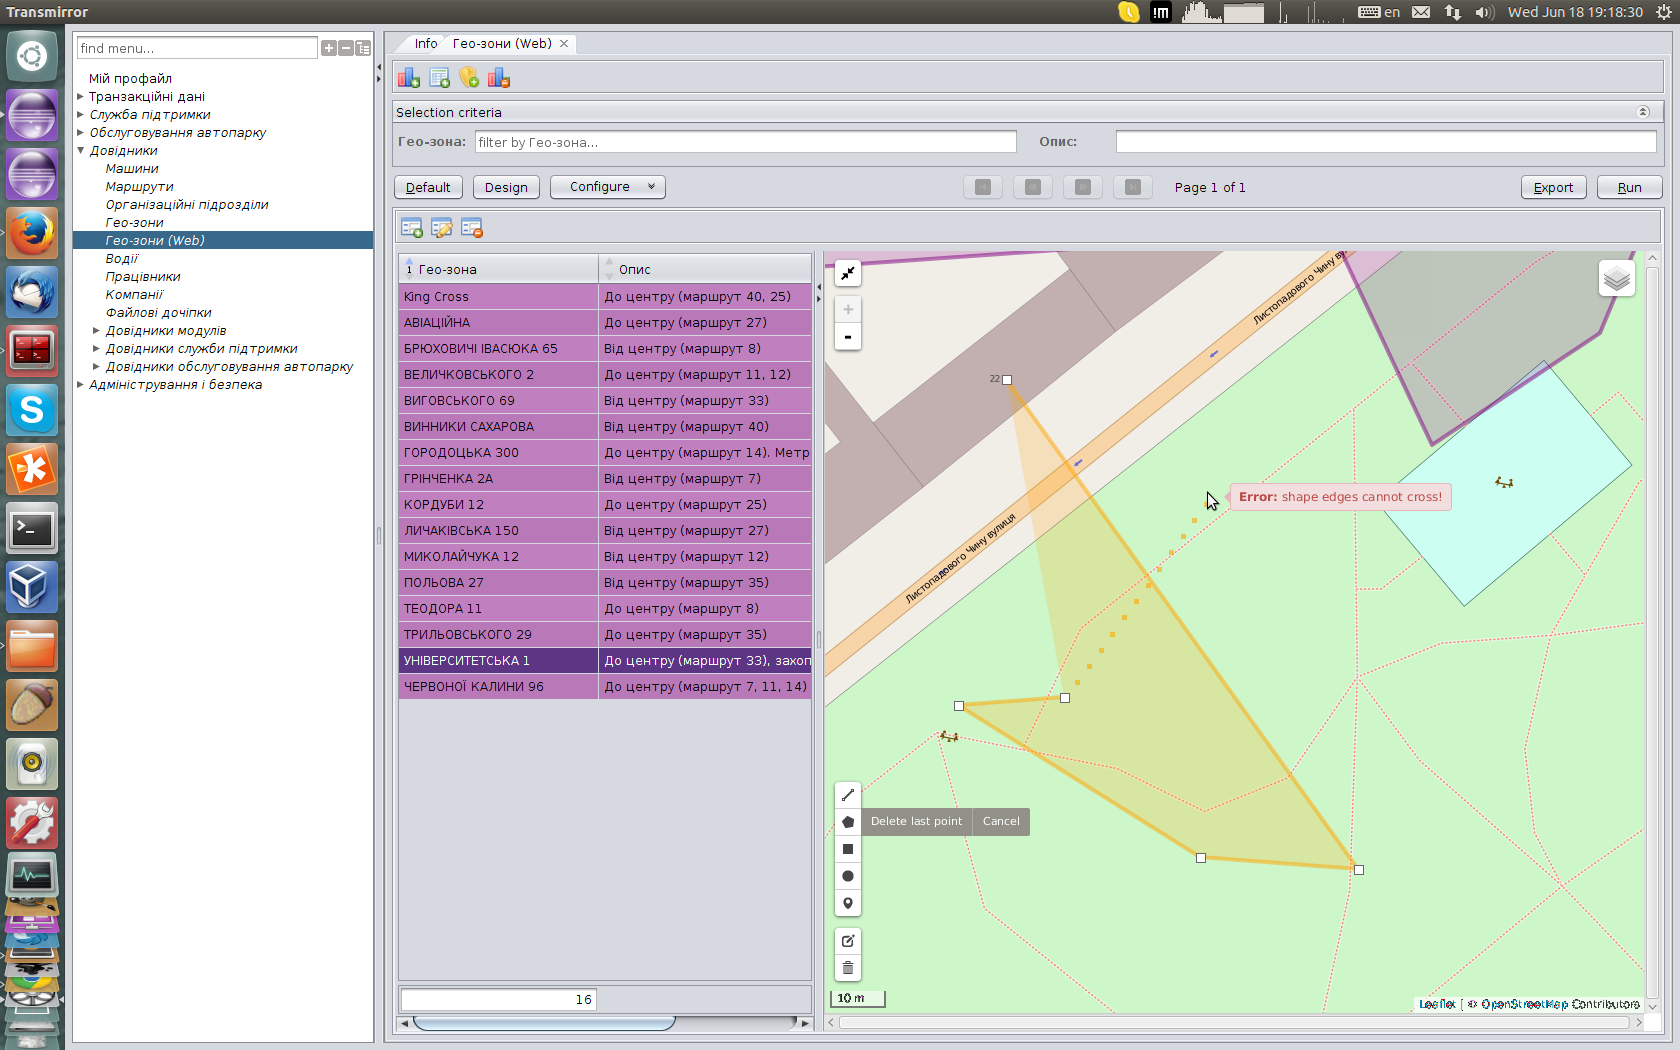
\includegraphics[width=\linewidth]{chapters/01-geozones/images/08-validation-for-complex-polygonial-geozone.png}
\caption{Validation for complex polygonial Geo-zone}\label{fig:08}
\end{figure}

\newpage
Map service changing is easily done by clicking on right top button. Basically tile services are not limited only by OpenStreetMap, Google, Yandex and Landscape, but at this stage only those are supported (figure~\ref{fig:09}). Please also note that several types of tiles for the same provider is available (for e.g. Sattelite, Roadmap or Terrain).

\begin{figure}[H]
\centering
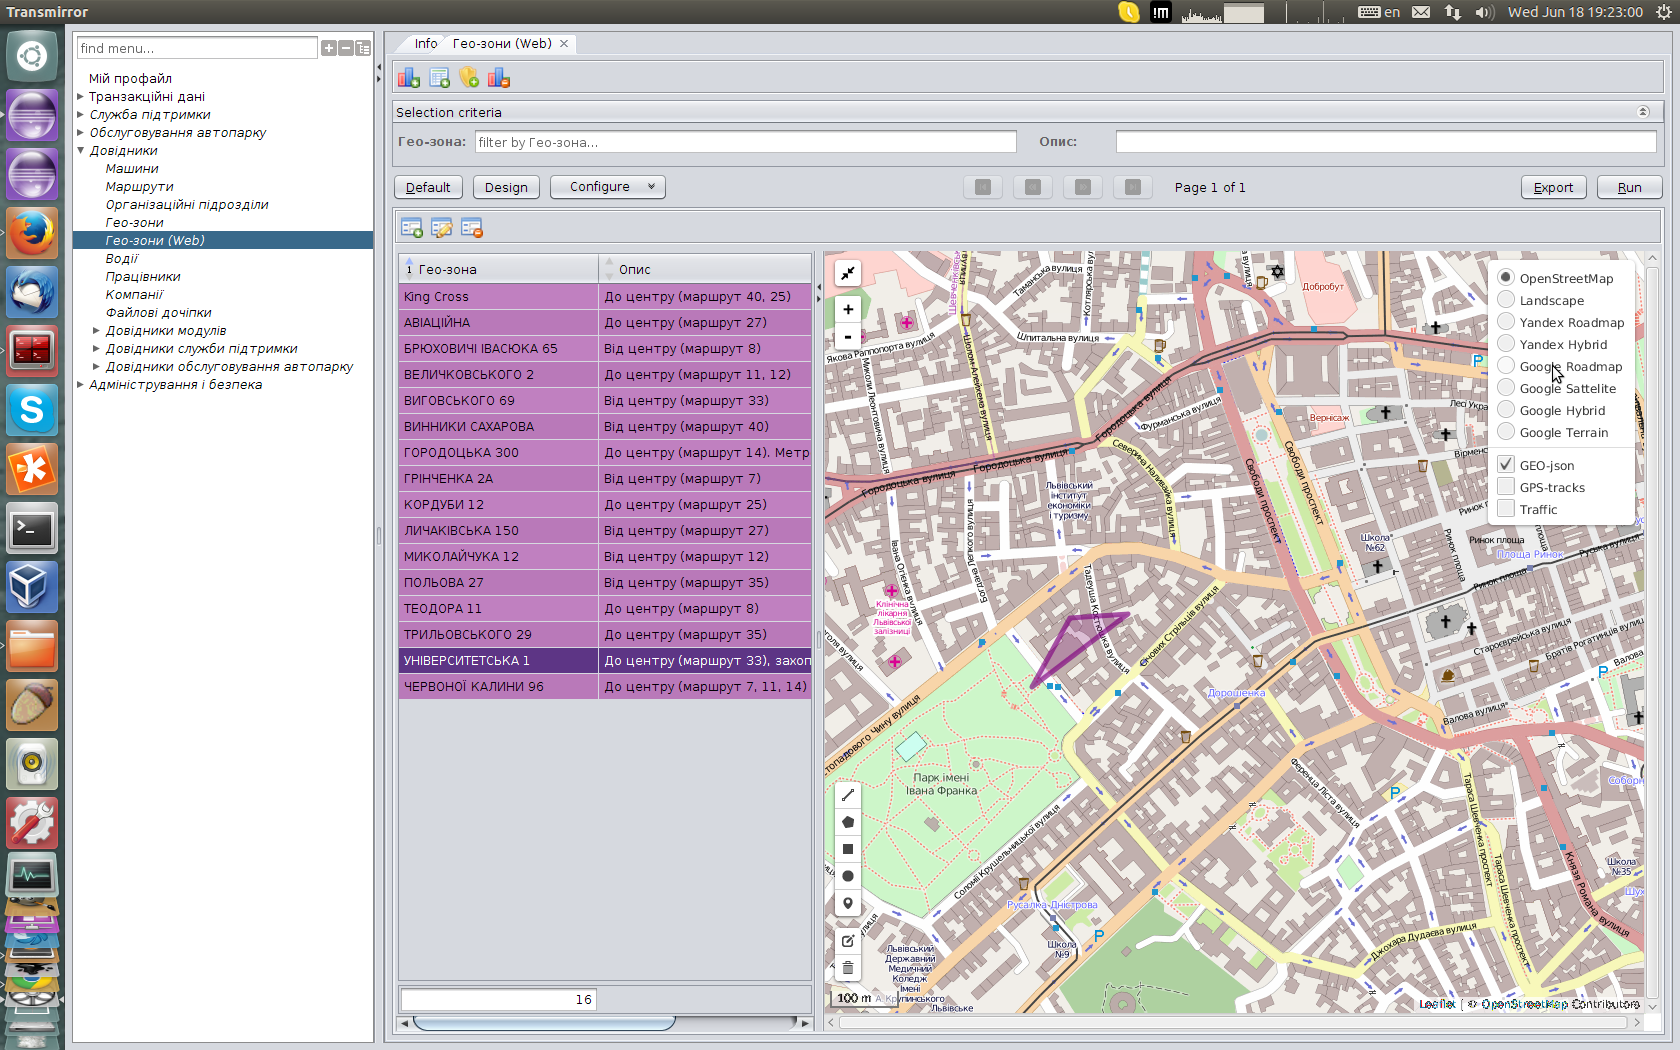
\includegraphics[width=\linewidth]{chapters/01-geozones/images/09-changing-map-tiling-service.png}
\caption{Changing map tiling service}\label{fig:09}
\end{figure}

\newpage
The result of map changing to Google Roadmap from OpenStreetMap.

\begin{figure}[H]
\centering
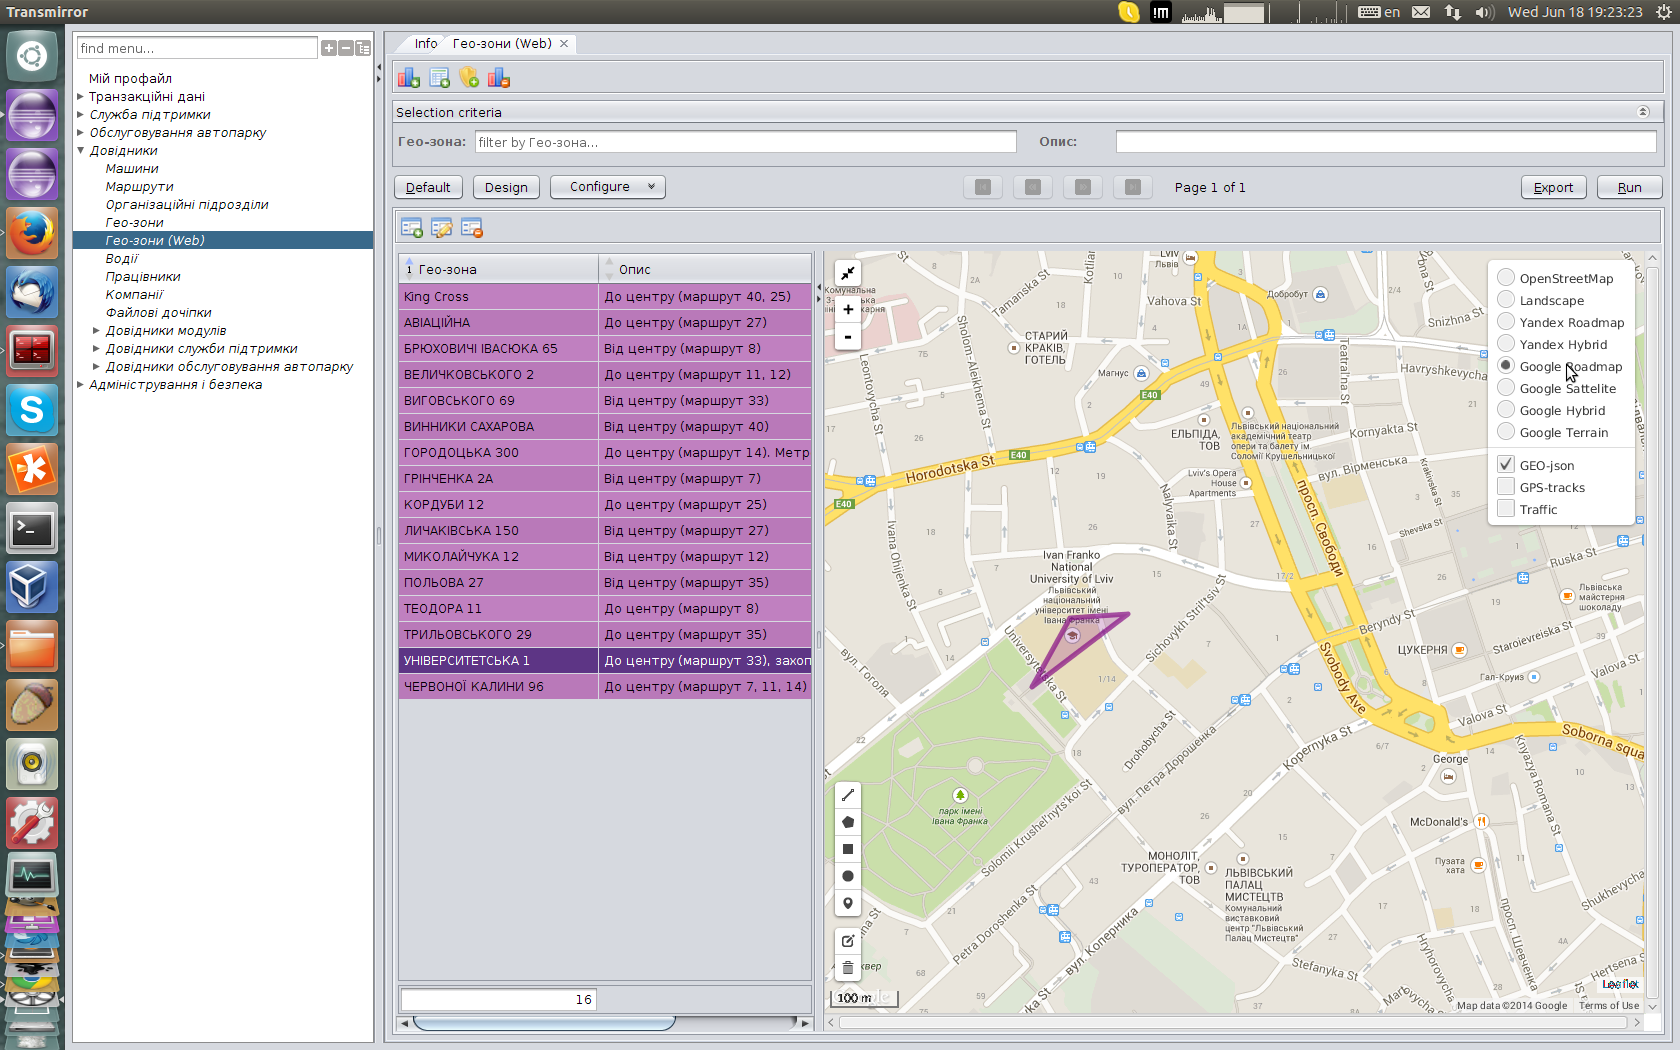
\includegraphics[width=\linewidth]{chapters/01-geozones/images/10-changed-map-tiling-service.png}
\caption{Changed map tiling service to Google Roadmap}\label{fig:10}
\end{figure}